\documentclass{beamer}
%\documentclass[handout,xcolor=svgnames]{beamer} %Version imprimible
%[9pt,xcolor=svgnames]

% -------------------------------------------------------------------
\usepackage{colores}
\usepackage{paquetes}
% \usepackage{licencia}
% \usepackage{pygments}

% -------------------------------------------------------------------
% \usepackage{modo}

% -------------------------------------------------------------------
\title{Documentación de proyectos con Doxygen}
\author{José Tomás Tocino García \\ \texttt{josetomas.tocino@uca.es}}
\date{16 de marzo de 2011}

\lstset{style=C++}

\begin{document}

% Transparencia de título
\begin{frame}
  \titlepage
\end{frame}

\normalsize
 
%Transparencia de índice
% \begin{frame}[Índice]
%  \frametitle{Índice} 
%  \transboxin
%  \tableofcontents
% \end{frame}

\begin{frame}{¿Qué es Doxygen?}
  \begin{center}
    {\Large\textbf{Doxygen} es una herramienta de generación automática de
    documentación.}
  \end{center}
  Es capaz de leer el código y documentarlo desde cero o ayudado
  de una sintaxis especial, muy sencilla, que aprenderemos aquí.

  \bigskip

  Funciona con muchos lenguajes: C, C++, Java, PHP, Python, VHDL...

  \bigskip

  El resultado también puede mostrarse en muchos formatos: en forma de web HTML,
  como un documento PDF, etcétera.

\end{frame}

\begin{frame}{Elementos que conforman Doxygen}
  \begin{center}
    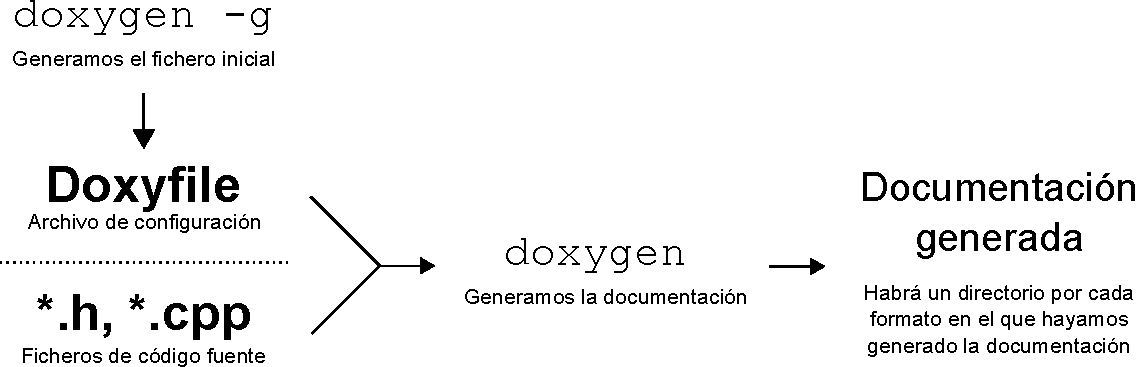
\includegraphics[width=\textwidth]{dibujo1}
  \end{center}
  
  \begin{itemize}
  \item Doxygen viene en los repositorios de la mayoría de distribuciones:\\
    \texttt{sudo apt-get install doxygen}
  \item El fichero \texttt{doxyfile} guarda las opciones de configuración. Por
    defecto se genera en formato HTML y \LaTeX.
  
  \end{itemize}
\end{frame}

\begin{frame}{Principales opciones del fichero de configuración}
  \begin{itemize}
  \item Nombre del proyecto: \\ 
    \texttt{PROJECT\_NAME = SecretProject}
  \item Idioma de la interfaz: \\ 
    \texttt{OUTPUT\_LANGUAGE = English (*)}
  \item Archivos a leer: \\
    \texttt{INPUT =  \\ FILE\_PATTERNS = }
  \item Extraer todo: \\
    \texttt{EXTRACT\_ALL = YES \\ }
  \item Formatos a generar: \\
    \texttt{GENERATE\_HTML = YES}
  \item Usar Graphviz para generar los diagramas: \\
    \texttt{HAVE\_DOT = YES}
  \item Descripción breve, termina con un punto: \\
    \texttt{JAVADOC\_AUTOBRIEF = YES}
  \end{itemize}
\end{frame}


\begin{frame}[fragile=singleslide]{Sintaxis básica para documentar el código}
  Los comentarios que Doxygen interpreta como documentación tienen una sintaxis
  especial. Siempre se colocan justo antes del código que queramos documentar.

  \medskip

  Las sintaxis más habituales son los comentarios con tres barras:

\begin{lstlisting}
/// Esto es un comentario de Doxygen
\end{lstlisting}

  \medskip

  O los comentarios en bloque con \textbf{dos asteriscos} de inicio:

\begin{lstlisting}
/**
  * Esto es un comentario de bloque
  */
\end{lstlisting}
  \medskip

\end{frame}

\begin{frame}{Partes de la documentación de un elemento}
  Doxygen divide la documentación de los elementos en tres partes:
  \begin{enumerate}
  \item \textbf{Descripción corta}: en una línea, explicar brevemente el código.
  \item \textbf{Descripción larga}: párrafo con varias líneas con una
    explicación más extensa. Hay que dejar un salto de línea para indicar el
    comienzo de la descripción larga. 


    Si tenemos activado \texttt{JAVADOC\_AUTOBRIEF = YES}, la descripción larga
    comienza tras el primer punto en los comentarios tipo \texttt{/** ... */}
  \item \textbf{Elementos adicionales}: podemos documentar, por ejemplo, para
    qué sirve cada parámetro de entrada, o qué valores devuelve la función,
    etc. Utilizaremos unos comandos del estilo @brief, @param, @return...
  \end{enumerate}
\end{frame}

\begin{frame}[fragile=singleslide]{Un ejemplo}

\begin{lstlisting}
/// Representa una ventana. 
/// Esto es la descripcion detallada
class Ventana{
public:
    /// Abre la ventana. 
    /// Las bisagras deben estar bien engrasadas.
    void Abrir();

    /// Color de la ventana.
    int color;
};
\end{lstlisting}
\end{frame}

\begin{frame}[fragile=singleslide]{Un ejemplo}
Mismo ejemplo, pero sintaxis alternativa
\begin{lstlisting}
/** 
 * @brief Representa una ventana. 
 * 
 * Esto es la descripcion detallada.
 */
class Ventana{
public:
    /**
     * @brief Abre la ventana.
     *
     * Las bisagras deben estar bien engrasadas.
     */
    void Abrir();

    /** Color de la ventana */
    int color;
};
\end{lstlisting}
\end{frame}


\begin{frame}[fragile=singleslide]{Elementos adicionales}
Los elementos adicionales aportan mucha información:
\begin{lstlisting}
    /**
     * @brief Cierra la ventana.
     *
     * Permite indicar la velocidad a la que 
     * cerrar la ventana.
     *
     * @param v Velocidad a la que se cierra.
     * 
     * @return true si la ventana se ha roto 
     * del portazo.
     *
     */
    bool Cerrar(float v);
\end{lstlisting}
\end{frame}

\begin{frame}[fragile=singleslide]{Elementos adicionales}
  Hay una lista inmensa de comandos que podemos usar además de los ya vistos:

  \begin{itemize}
  \item \texttt{@author}: autor del código.
  \item \texttt{@date}: fecha.
  \item \texttt{@exception}: posibles excepciones que lanza el método.
  \item \texttt{@todo}: elementos pendientes en la lista TO-DO.
  \item Podemos agrupar elementos: 
\begin{lstlisting}
    /// @{
    /// @name Coordenadas de las ventanas
    float x;
    float y;
    /// @}

\end{lstlisting}
  \end{itemize}
  
\end{frame}

\begin{frame}{Chimpón}
  \begin{center}
{\Large
    ¿Preguntas? }
  \end{center}
\end{frame}
\end{document}
  
